\documentclass[conference]{IEEEtran}
\IEEEoverridecommandlockouts
% The preceding line is only needed to identify funding in the first footnote. If that is unneeded, please comment it out.
\usepackage{cite}
\usepackage{amsmath,amssymb,amsfonts}
\usepackage{algorithm}
\usepackage{algpseudocode}
\usepackage{graphicx}
\usepackage{textcomp}
\usepackage{xcolor}
\usepackage{hyperref}
\hypersetup{
    colorlinks=true,
    linkcolor=magenta,
    citecolor=green,  % Change this to your desired citation color
    urlcolor=blue
}
\pagestyle{plain}

\def\BibTeX{{\rm B\kern-.05em{\sc i\kern-.025em b}\kern-.08em
    T\kern-.1667em\lower.7ex\hbox{E}\kern-.125emX}}
\begin{document}

\title{Towards Culturally-Aware Text-to-Image Generation: Dataset Taxonomy and a Vietnamese Diffusion Model Pipeline}
%{\footnotesize \textsuperscript{*}Note: Sub-titles are not captured in Xplore and should not be used}
% \thanks{Identify applicable funding agency here. If none, delete this.}

\author{\IEEEauthorblockN{1\textsuperscript{st} Van Quang Nghiem}
\IEEEauthorblockA{\textit{Viettel AI \& Data Services Center} \\
Hanoi, Vietnam \\
quangnv60@viettel.com.vn}
}

\maketitle

\begin{abstract}
Text-to-image (T2I) generation is a rapidly evolving field in computer vision and natural language processing, enabling the automatic creation of images from textual descriptions. In this paper, we present a comprehensive survey of existing T2I datasets and benchmark tasks, focusing on the diversity of public datasets and the role of image captioning in prompt synthesis. Beyond the survey, we propose a novel taxonomy that categorizes T2I datasets based on language, domain, and annotation characteristics to support research in both English and low-resource languages. Furthermore, we introduce a Vietnamese-specific generation pipeline based on diffusion models, which integrates language-specific preprocessing and cultural context adaptation. Our work provides a solid foundation and practical guidance for future studies aiming to improve T2I generation in multilingual and culturally rich settings.
\end{abstract}

\begin{IEEEkeywords}
Text-to-Image Generation; Dataset Survey; Taxonomy; Diffusion Model; Vietnamese Language; Multimodal Learning; Prompt Engineering
\end{IEEEkeywords}

\section{Introduction}
In recent years, generative models have become a cornerstone of modern artificial intelligence, demonstrating remarkable capabilities across various domains such as text generation, image synthesis, and multimodal understanding. These models are largely empowered by advancements in deep learning architectures, particularly the Transformer \cite{vaswani2023attentionneed}, which has laid the foundation for state-of-the-art performance in both language and vision-related tasks.

Image generative models—including Variational Autoencoders (VAEs) \cite{vae}, Generative Adversarial Networks (GANs) \cite{gans}, and diffusion models like Stable Diffusion \cite{stablediffusion} and OpenAI's DALL·E 3 \cite{openai2023dalle3}—have revolutionized the way machines generate high-fidelity, realistic visuals. On the language side, models such as OpenAI's GPT series \cite{openai2023gpt4} and Google's Gemini \cite{google2023gemini} showcase unprecedented fluency and contextual awareness in natural language generation. Meanwhile, the emergence of multimodal models, often referred to as Vision-Language Models (VLMs)—such as CLIP \cite{clip}, Flamingo \cite{alayrac2022flamingo}, and GPT-4 Vision \cite{openai2023gpt4}—enables AI systems to reason across both text and images, marking a significant leap toward generalized intelligence.

These generative models can be categorized into two main types: open-source models (e.g., Stable Diffusion, LLaMA \cite{touvron2023llama}, Qwen \cite{yang2024qwen2}, InternLM \cite{chen2024internvl}) and closed-source commercial models (e.g., DALL·E 3, Midjourney, GPT-4, Gemini). Each category offers distinct advantages—open-source models provide flexibility for customization and research, while commercial models often deliver cutting-edge performance through proprietary optimization and large-scale training.

Among these, image generation remains one of the most impactful and widely discussed applications globally. Despite this progress, a notable challenge arises when adapting these technologies to non-English and non-Chinese linguistic and cultural contexts—particularly for Vietnamese. Most current generative models are developed and fine-tuned primarily for English or Chinese, limiting their effectiveness when applied to Vietnamese text inputs. Although there have been efforts to create Vietnamese language models such as PhoBERT \cite{nguyen2020phobertpretrainedlanguagemodels} and VinTERN 3.5 \cite{doan2024vintern1befficientmultimodallarge} (built on Qwen 2.0.5B Instruct \cite{yang2024qwen2} and InternViT-300M-448px \cite{chen2024internvl}), these initiatives primarily focus on text understanding or multimodal capabilities with minimal advancement in Vietnamese-specific image generation.

This report proposes a comprehensive solution to address this gap by building a Vietnamese-centered image generation pipeline. It includes constructing a culturally and linguistically representative dataset, selecting and training suitable generative models, and establishing a benchmark to evaluate performance. Our goal is to develop a system that not only understands Vietnamese prompts accurately but also generates images aligned with Vietnam's cultural identity and visual aesthetics.

The remainder of this article is organized as follows: Section \ref{sec:relatedwork} reviews related work in the domains of generative models, Vietnamese datasets, and multimodal learning. Section \ref{sec:medthods} details our proposed approach, including the taxonomy construction and the Vietnamese-specific generation pipeline. Finally, Section \ref{sec:conclusion} presents our conclusions and outlines future work directions.


\section{Related Work}
\label{sec:relatedwork}
In this section, we analyze related works, including text-to-image (T2I) datasets, benchmarks, image captioning models (used for prompt synthesis), and models for the T2I task.

\subsection{Datasets}
This subsection is divided into two parts: first, an overview of popular public datasets commonly used for T2I tasks; second, a presentation of some Vietnamese datasets.

\subsubsection{General Public Datasets}
Datasets are crucial for training, evaluating, and ensuring fairness in T2I models. Large-scale datasets enhance image generation capabilities. Table~\ref{table_dataset} summarizes key datasets in this field.


\begin{table*}[h]
	\centering
	\caption{Datasets in the T2I task.}
	\label{table_dataset}
	\resizebox{0.5\linewidth}{!}{
	\begin{tabular}{@{}llll@{}}
		\hline
		\textbf{Dataset} & \textbf{Year} & \textbf{Size} & \textbf{Source} \\ \hline
		Oxford 102 Flower Dataset\cite{nilsback2008automated} & 2008 & 8,189 & University of Oxford \\
		UIUC Pascal Sentence\cite{rashtchian2010collecting} & 2010 & 1,000 & VOC2008 \\
		SBU Captions\cite{ordonez2011im2text} & 2011 & 1,000,000 & Flickr.com \\
		Flickr8K\cite{plummer2016flickr30kentitiescollectingregiontophrase} & 2013 & 8,092 & Flickr.com \\        COCO\cite{lin2014microsoft} & 2014 & 330,000+ & Microsoft \\       
		ABSTRACT-50S\cite{vedantam2015cider} & 2015 & 500 & ASD \\
		Flickr30k\cite{plummer2016flickr30kentitiescollectingregiontophrase} & 2015 & 31,783 & Flickr.com \\
		COCO Captions\cite{chen2015microsoftcococaptionsdata} & 2015 & 204,721 & Microsoft \\
		PASCAL-50S\cite{vedantam2015cider} & 2015 & 1,000 & VOC2008 \\
		vQA\cite{antol2015vqa} & 2015 & 254,721 & MS COCO \& Abstract Images \\        Pinterest40M\cite{kazemi2017show} & 2016 & 40,000,000 & Pinterest.com \\
		Visual Genome\cite{krishna2017visual} & 2017 & 108,000 & Stanford University \\
		vQAv2.0\cite{goyal2017making} & 2017 & 204,721 & MS COCO \\        CelebA\cite{zhang2019showattendtranslateunpaired} & 2018 & 202,599 & Chinese University of Hong Kong \\
		Nocaps\cite{agrawal2019nocaps} & 2019 & 15,100 & Open Images V4 (Flickr.com) \\
		VCR\cite{zellers2019recognition} & 2019 & 110 & LSMDC \& YT \\
		Conceptual Captions\cite{sharma2018conceptual} & 2018 & 3,369,218 & Google Research \\
		LAION-400M\cite{schuhmann2021laion400m} & 2021 & 400,000,000 & LAION (Large-scale AI Open Network) \\
		CC-500\cite{feng2024cc500} & 2022 & 500 & Synthetic prompts \\
		Conceptual 12M\cite{changpinyo2021cc12m} & 2021 & 12,423,374 & World Wide Web \\
		LAION-5B\cite{schuhmann2021laion400m} & 2022 & 5,000,000,000 & LAION \\
		DiffusionDB\cite{wang2022diffusiondb} & 2022 & 2,000,000 & Open-source contributions \\
		Winoground\cite{bitton2022winoground} & 2022 & 800 & Getty Images API \\
		DrawBench\cite{saharia2022photorealistic} & 2022 & 200 & DALL-E \& Reddit \\
		ABC-6K\cite{zhang2024abc6k} & 2022 & 6,400 & MS COCO \\
		I2P\cite{schramowski2023safelatentdiffusionmitigating} & 2023 & 4,703 & User generated prompts \\
		T2I-CompBench\cite{huang2023t2icompbench} & 2023 & 6,000 & Generated prompts by GPT \\         PaintSkills\cite{cho2023dallevalprobingreasoningskills} & 2023 & 65,535 & Synthetic prompts \\
		RichHF-18K\cite{liang2023richhf} & 2024 & 18,000 & Pick-a-Pic \\
		MARIO-10M\cite{chen2023textdiffuser} & 2024 & 10,061,720 & LAION, TMDB, Open Library \\
		\hline
	\end{tabular}
}
\end{table*}

The COCO dataset \cite{chen2015microsoftcococaptionsdata} contains over 300,000 images, each with five human-generated captions covering diverse objects and scenes. It is widely used for image annotation, generation, and retrieval.

Flickr30k \cite{plummer2016flickr30kentitiescollectingregiontophrase} and Flickr8k \cite{plummer2016flickr30kentitiescollectingregiontophrase} provide thousands of images with multiple user-generated descriptions, supporting image generation and retrieval tasks.

The Oxford 102 Flower dataset \cite{nilsback2008automated} focuses on fine-grained image generation for 102 flower species with detailed descriptions.

The Conceptual Captions dataset \cite{changpinyo2021conceptual12m} offers millions of image-caption pairs gathered from the web, emphasizing conceptual understanding for multimodal learning.

Large-scale datasets like LAION-400M \cite{schuhmann2021laion400m} and LAION-5B \cite{schuhmann2021laion400m} provide hundreds of millions to billions of image-text pairs, enabling training of large T2I models such as CLIP.

Other datasets such as Visual Genome \cite{krishna2017visual} and SBU Captions \cite{ordonez2011im2text} offer region-level annotations and contextual captions, enriching model capabilities.

Specialized datasets like DiffusionDB \cite{wang2022diffusiondb} and PaintSkills \cite{cho2023dallevalprobingreasoningskills} focus on prompt diversity and artistic image generation, respectively.

Vietnamese datasets will be discussed in the following subsection.

\subsubsection{Vietnamese public dataset}
In recent years, the advancement of multimodal artificial intelligence, particularly in tasks such as image captioning and vision-language question answering (VQA), has highlighted the importance of high-quality language-specific datasets. For Vietnamese, a low-resource language, the availability of annotated image-caption datasets and OCR-based VQA corpora remains limited, which poses challenges for training robust models that can generalize across diverse contexts.
\begin{table*}[t]
	\centering
	\caption{Overview of Vietnamese Image Captioning and OCR-VQA Datasets}
	\resizebox{00.8\linewidth}{!}{%
		\begin{tabular}{|p{3.2cm}|c|c|p{6.4cm}|}
			\hline
			\textbf{Dataset Name} & \textbf{\#Images} & \textbf{\#Captions / QA pairs} & \textbf{Description} \\
			\hline
			KTVIC \cite{pham2024ktvic} & 4,327 & 21,635 (5/img) & Manually written Vietnamese captions; covers various daily-life scenes. \\
			\hline
			UIT-ViIC \cite{lam2020uitviic} & 3,850 & 19,250 (5/img) & Sports-related images from MS COCO; among the first captioning datasets for Vietnamese. \\
			\hline
			UIT-OpenViIC \cite{bui2023uitopenviic} & $\sim$3,000 & $\sim$15,000 & Real-world scenes in Vietnam with culturally contextualized captions. \\
			\hline
			Vietnamese COCO 2017 \cite{dinhanhx_VisualRoBERTa_2022} & 118,000 (train+val) & $\sim$590,000 & Machine-translated from English COCO using VinAI Translate. \\
			\hline
			Flickr8k Vietnamese & 8,000 & 40,000 & Automatically translated from Flickr8k; useful for small-scale training. \\
			\hline
			Viet-OCR-VQA (5CD-AI) \cite{doan2024vintern1befficientmultimodallarge} & $\sim$3,000 & $\sim$12,000 & OCR-based VQA dataset with real-world scanned images. \\
			\hline
			ViOCRVQA \cite{pham2024viocrvqa} & 28,282 & 123,781 & OCR-VQA dataset on various documents. Introduced in: \textit{ViOCRVQA: Novel Benchmark Dataset and Vision Reader for Vietnamese VQA}. \\
			\hline
			4,995 Vietnamese OCR Images Dataset \cite{nexdata2024vietnameseocr} & 4,995 & N/A & 258 natural scene images, 2,553 internet images, and 2,184 document scans. Annotated with line/column bounding boxes and text. Accuracy $>$97\%. \\
			\hline
		\end{tabular}%
	}
	\label{tab:vietnamese_datasets}
\end{table*}


Several initiatives have addressed this gap by constructing Vietnamese image captioning datasets. One of the earliest is \textbf{UIT-ViIC} \cite{lam2020uitviic}, derived from MS COCO images focused on sports, containing 3,850 images annotated with five human-written Vietnamese captions per image. This dataset laid the foundation for evaluating Vietnamese captioning models. Similarly, \textbf{KTVIC} \cite{pham2024ktvic} expands the context to everyday life scenes, consisting of 4,327 images and over 21,000 captions, written manually to reflect natural and contextual Vietnamese.

Another significant contribution is \textbf{UIT-OpenViIC} \cite{bui2023uitopenviic}, which includes complex real-world scenes captured in Vietnam. This dataset emphasizes the diversity and cultural richness of Vietnamese environments and is particularly valuable for fine-tuning large captioning models on localized data. In addition to manually created datasets, translated datasets such as \textbf{Vietnamese COCO 2017} \cite{dinhanhx_VisualRoBERTa_2022} and \textbf{Flickr8k Vietnamese} have extended existing English caption corpora into Vietnamese using automatic translation systems, notably VinAI Translate. Although these help increase the scale, their reliance on machine translation may introduce noise or unnatural phrasing.

Despite these efforts, current Vietnamese image captioning datasets are still relatively few in number and lack diversity in both visual content and captioning styles. Most datasets focus on narrow domains (e.g., sports or daily life) and offer limited generalization across complex, real-world visual-linguistic reasoning.

Beyond captioning, OCR-based VQA has emerged as a vital task, especially for digitizing and understanding documents in Vietnamese. The \textbf{Viet-OCR-VQA} dataset by 5CD-AI \cite{doan2024vintern1befficientmultimodallarge} is a recent addition hosted on Hugging Face, featuring questions and answers grounded in OCR-detected content. Similarly, \textbf{ViOCRVQA} \cite{pham2024viocrvqa} introduces a novel benchmark with vision-reading capabilities that include documents, bills, and ID cards—paving the way for applying language-specific VQA models in administrative and legal domains. Another resource is the \textbf{4,995 Vietnamese OCR Images Dataset} \cite{nexdata2024vietnameseocr}, which provides annotated Vietnamese text in natural scenes, further supporting the development of Vietnamese OCR engines.

Nevertheless, these OCR-VQA datasets remain fragmented and relatively small-scale. There is a need for standardized benchmarks with unified annotation guidelines and broader domain coverage to enable fair comparisons and reproducibility across models.

\noindent While there are several publicly available datasets for image captioning and visual question answering, the \textbf{majority} of them are in \textbf{English}. Only a \textbf{limited number} of datasets provide \textbf{Vietnamese-language} captions or QA pairs. Although it is possible to apply \textbf{machine translation} or \textbf{large language models (LLMs)} to convert English annotations into Vietnamese, the resulting captions often lack \textbf{cultural nuances} and \textbf{local context} that are essential for building more meaningful Vietnamese AI systems. Therefore, it is \textbf{crucial} to develop a \textbf{native Vietnamese dataset} that authentically reflects \textbf{Vietnamese culture} in both \textbf{images} and \textbf{captions}.


\subsection{Image Captioning for Creating T2I Dataset}
\subsubsection{Image captioning}
In recent years, the task of image captioning has increasingly leveraged powerful \textbf{vision-language models (VLMs)} and \textbf{vision-language large models (VLLMs)}. These models combine the capability of understanding visual content and generating contextually relevant, coherent text, making them well-suited for generating diverse and natural captions. This process plays a crucial role in building high-quality \textbf{text-to-image (T2I)} datasets, where caption diversity and visual fidelity are both essential.

Several representative models have been widely adopted or explored for this task:

\begin{itemize}
	\item \textbf{BLIP/BLIP-2} \cite{li2023blip2}: Open-source frameworks designed specifically for vision-language tasks, known for strong performance on both captioning and VQA tasks. However, their multilingual capacity—especially for Vietnamese—is still limited without additional fine-tuning.
	
	\item \textbf{GPT-4V} \cite{openai2023gpt4}: A closed-source, commercial VLLM developed by OpenAI that shows impressive capability in generating captions that are \textbf{rich in detail}, often identifying both \textbf{locations} and \textbf{cultural elements} (e.g., “Hoan Kiem Lake”, “ao dai”). Nonetheless, its use is restricted due to \textbf{API cost} and lack of open access.
	
	\item \textbf{Gemini 2.5 Flash/Pro} \cite{google2023gemini}: Another commercial model with multilingual support and good captioning abilities, though it tends to provide \textbf{less specific context} compared to GPT-4V. Moreover, it suffers from the same closed-access limitations.
	
	\item \textbf{Qwen2.5-VL-7B-Instruct} \cite{yang2024qwen2}: An open-source vision-language model that supports Vietnamese. It can interpret image content and generate coherent captions. However, due to being \textbf{not trained on culturally specific Vietnamese datasets}, it often lacks understanding of Vietnamese locations or attire.
	
	\item \textbf{Vi-VLM/Vistral-V-7B} \cite{vistral2024vietnamese}: A recent Vietnamese-finetuned open-source model that demonstrates strong potential. It recognizes common Vietnamese landmarks (e.g., Ho Guom), attire (ao dai), and context, due to being \textbf{specifically trained on Vietnamese datasets}. This direction appears to be the most \textbf{feasible and scalable}, as such models can be further improved using \textbf{LoRA}, \textbf{QLoRA}, \textbf{PEFT}, or full fine-tuning—without requiring enormous hardware.
\end{itemize}

\textbf{Comparison Example.} Below is a qualitative comparison of image captioning outputs from different models (see Figure~\ref{fig:reviewvllmcaptioning}) on a set of Vietnamese cultural images:

\begin{itemize}
	\item \textbf{GPT-4V} provides \textbf{highly descriptive and culturally aware} captions. It recognizes Ho Guom, ao dai, Ha Noi, and the setting, producing natural, human-like captions. Its drawback is high cost and lack of openness.
	
	\item \textbf{Gemini 2.5} models produce grammatically correct captions but are \textbf{less contextualized}. The captions tend to generalize visual features and may not fully capture the Vietnamese context.
	
	\item \textbf{Qwen2.5-VL} shows good image understanding and supports Vietnamese prompts. However, due to \textbf{limited exposure to Vietnamese cultural data}, it often fails to recognize landmarks or local attire correctly.
	
	\item \textbf{Vistral-V-7B}, being \textbf{finetuned on Vietnamese datasets}, generates captions with better cultural alignment. It can name Kinh Thanh Hue, recognize Cho Noi, and describe scenes in a Vietnamese way. Its open-source nature also makes it suitable for further development.
\end{itemize}

\begin{figure*}[h!]
	\centering
	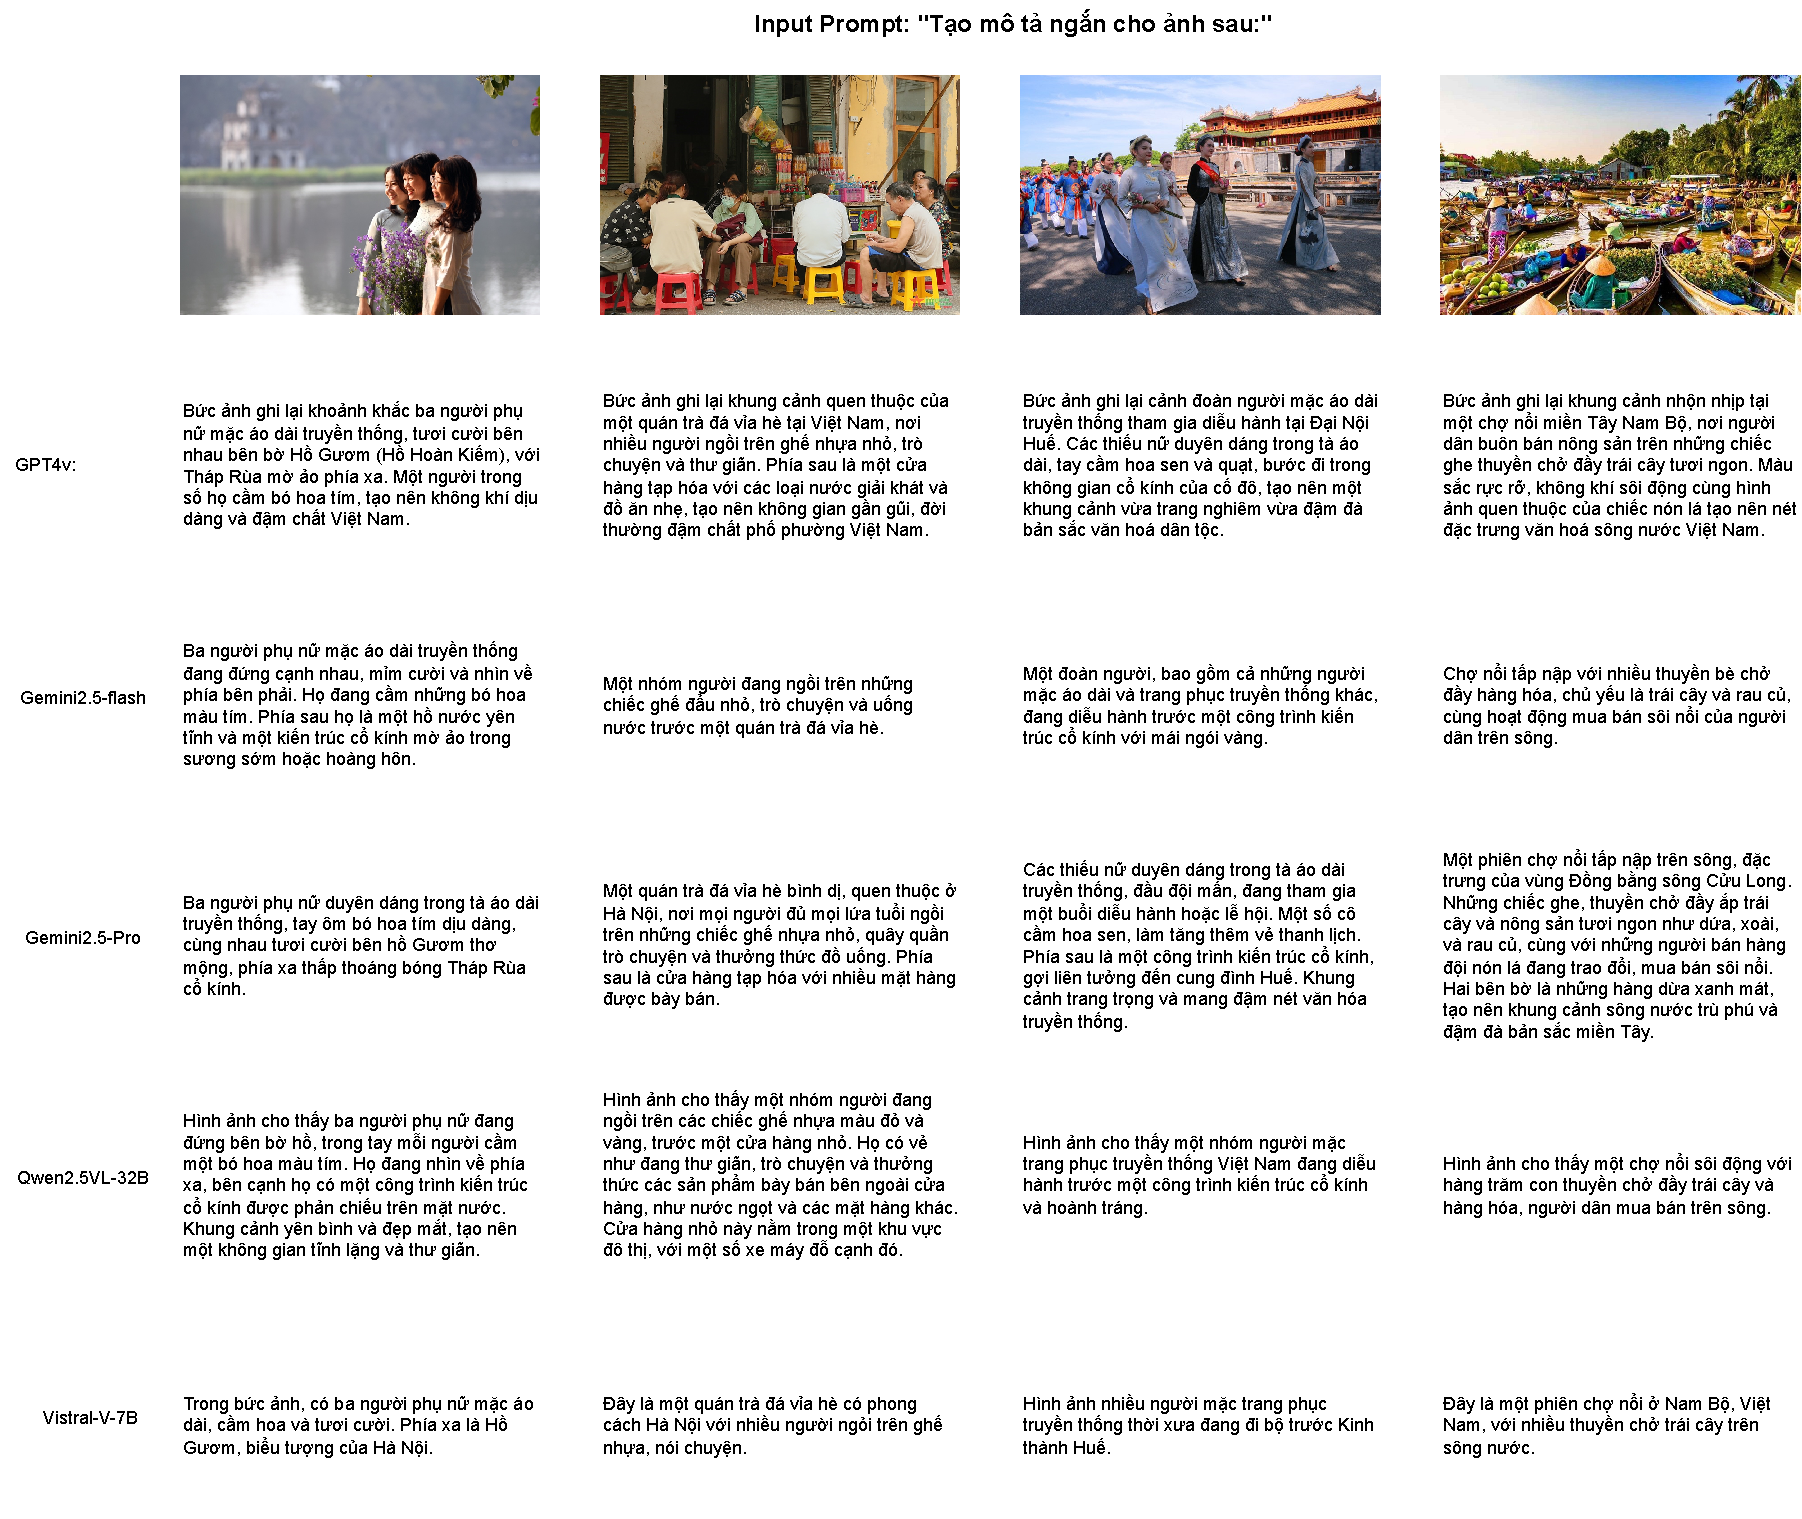
\includegraphics[width=1\textwidth]{captioningreview.pdf} % Add the file name for your figure here
	\caption{Fine-Tuning Process Overview}
	\label{fig:reviewvllmcaptioning}
\end{figure*}


\subsubsection{OCR Image Captioning}
Optical Character Recognition (OCR) plays an important role in image captioning, particularly when dealing with images that contain textual content. Understanding the embedded text in images allows for more accurate and meaningful captions, which is crucial when constructing high-quality text-to-image (T2I) datasets. This is especially relevant for applications such as generating advertisement posters or propaganda-style images, where text is a core part of the visual design.

Traditional OCR pipelines for Vietnamese have seen significant development. Among the most effective approaches are models fine-tuned from PaddleOCR
\cite{paddleocr2021} for Vietnamese, or systems that combine PaddleOCR with VietOCR \cite{vietocr2020} to extract both textual content and its corresponding bounding boxes. However, these conventional systems often assume consistent layouts or fixed formats, which limits their scalability for large-scale, diverse datasets where image structures vary significantly.

Recently, vision-language models (VLMs) have emerged as promising alternatives. For example, Vintern-1B-v2 \cite{doan2024vintern1befficientmultimodallarge} is a compact VLM with only one billion parameters, yet demonstrates impressive performance on OCR and VQA tasks for Vietnamese inputs. While this model excels at extracting text and preserving its visual structure, it lacks the capability to return precise bounding box coordinates for the detected text.

On the other hand, larger models such as GPT-4V, Gemini 2.5, or Qwen-VL-72B are capable of handling both OCR and spatial localization tasks. These models can not only recognize and understand text in images but also provide coordinates for each text span. The trade-off, however, lies in their cost — either requiring API calls or significant hardware resources for on-premise deployment.

Nevertheless, the high OCR capability of modern VLMs makes them viable tools for developing OCR-aware image captioning systems, which are essential in constructing robust T2I datasets that include embedded textual elements.

\subsection{Text to Image generated model}


Modern text-to-image (T2I) generation models predominantly follow two architectural paradigms: diffusion-based models and autoregressive models. Each comes with its strengths, limitations, and implications when applied to low-resource languages like Vietnamese.

\subsubsection{Diffusion-based Models.} Diffusion models have become the mainstream approach for high-fidelity image synthesis. Prominent examples include \textbf{Stable Diffusion} \cite{stablediffusion}, \textbf{SDXL} \cite{stablediffusionxl2023}, and the upcoming \textbf{Stable Diffusion 3.5} \cite{stablediffusion35}, all of which are trained on large-scale English datasets. These models typically rely on a dual-encoder setup, where a text encoder (such as CLIP's text model) maps the input prompt into a latent space, which then guides the iterative denoising process to generate an image.

While these models can generate visually appealing content, they face challenges when applied to Vietnamese inputs. Several strategies have been explored to bridge this gap, such as replacing the English text encoder with a Vietnamese model like \textbf{PhoBERT} \cite{nguyen2020phobertpretrainedlanguagemodels}, or adapting the entire CLIP \cite{clip} backbone to a Vietnamese-compatible version. Although such methods improve the model's ability to interpret Vietnamese prompts, the \emph{latent space} of the pretrained diffusion model remains inherently biased towards English-language semantics. As a result, the generated images often fail to capture the unique cultural, contextual, and linguistic elements of Vietnamese.

A critical limitation of diffusion models—especially those based on the Stable Diffusion architecture—is their poor handling of \textbf{text rendering} within images. For example, when tasked with generating posters or flyers that require accurate Vietnamese text placement, these models often produce distorted or unreadable characters. This shortcoming hinders their direct applicability in design-oriented tasks such as advertising or educational content creation.

To address this, techniques such as \textbf{ControlNet} \cite{controlnet2023} have been introduced to guide the generation process using additional conditions (e.g., segmentation maps, pose skeletons, or text layouts). However, integrating such constraints still requires a multi-stage pipeline, often involving OCR extraction, layout specification, and fine-grained prompt engineering. Therefore, building a robust Vietnamese T2I system likely necessitates decomposing the problem into sub-tasks with modular solutions.

\subsubsection{Autoregressive Models.} On the other side of the spectrum, autoregressive models like \textbf{DALL·E} \cite{openai2023dalle3}, and newer research efforts such as \textbf{Flamingo} \cite{alayrac2022flamingo} and \textbf{FluX} \cite{yang2024158bitflux} (from OpenAI and other labs) adopt a token-by-token generation approach. These models often treat both text and images as sequences of discrete tokens and generate visual outputs in a left-to-right (or block-wise) manner.

Autoregressive models generally offer finer control over structure and layout and have shown greater promise in tasks requiring the faithful reproduction of text, logos, and graphical elements. However, they typically lag behind diffusion models in terms of photorealism and visual fidelity. Additionally, training such models requires massive computational resources and access to tokenized multi-modal datasets, which are often unavailable or limited for low-resource languages like Vietnamese.

Nonetheless, given their strength in layout-sensitive tasks, autoregressive models may provide a valuable foundation for future systems where text rendering and spatial alignment are critical — especially if adapted to incorporate Vietnamese tokenizer support and multilingual training objectives.

\subsubsection{Summary.} Overall, while diffusion models dominate in terms of popularity and image quality, their limitations in multilingual text rendering — especially Vietnamese — suggest the need for hybrid systems. Combining the strengths of both paradigms, possibly through modular pipelines or cross-modal fusion (e.g., CLIP-guided layout control combined with OCR-informed generation), could offer a viable path forward for generating Vietnamese-specific visual content with embedded text.

\subsection{Model Evaluation}

Evaluating the performance of vision-language models is essential for determining their quality, reliability, and suitability for downstream tasks. This section describes evaluation metrics and methodologies for three main components: Image Captioning, OCR, and Text-to-Image generation using diffusion models.

\subsubsection{Image Captioning Evaluation}

\paragraph{Automatic Metrics.} Image captioning models are typically evaluated using a set of standard metrics that compare the generated caption with human-written references. The most common include:

\begin{itemize}
	\item \textbf{BLEU (Bilingual Evaluation Understudy):} BLEU-n compares the n-gram precision between a candidate and reference captions. It is computed as:
	\begin{equation}
		\text{BLEU-n} = \text{BP} \cdot \exp\left( \sum_{n=1}^N w_n \log p_n \right)
	\end{equation}
	where $p_n$ is the modified n-gram precision, $w_n$ is a weight (usually $1/N$), and BP is the brevity penalty:
	\begin{equation}
		\text{BP} = 
		\begin{cases}
			1 & \text{if } c > r \\
			\exp(1 - \frac{r}{c}) & \text{if } c \leq r
		\end{cases}
	\end{equation}
	with $c$ and $r$ being the lengths of the candidate and reference captions.
	
	\item \textbf{METEOR:} This metric aligns unigrams based on exact, stemmed, or synonym matches. The score is computed as:
	\begin{equation}
		\text{METEOR} = F_{mean} \cdot (1 - Penalty)
	\end{equation}
	where $F_{mean}$ is the harmonic mean of unigram precision and recall, and Penalty depends on the number of chunks (non-contiguous matches).
	
	\item \textbf{CIDEr:} Weights n-gram similarity by TF-IDF across references:
	\begin{equation}
		\text{CIDEr}(c, S) = \frac{1}{|S|} \sum_{s \in S} \text{sim}_{tf-idf}(c, s)
	\end{equation}
	where $c$ is the candidate and $S$ the set of references.
	
	\item \textbf{SPICE:} Converts captions into scene graphs and compares tuples (object, attribute, relation).
	
	\item \textbf{CLIPScore:} Measures semantic similarity using CLIP embeddings:
	\begin{equation}
		\text{CLIPScore}(I, T) = \cos(\phi_I(I), \phi_T(T))
	\end{equation}
	where $\phi_I$ and $\phi_T$ are the CLIP image and text encoders.
\end{itemize}
\noindent\textbf{Example (BLEU-1):}
{\small
	\begin{verbatim}
Reference: ``A dog is playing with a ball.''
Candidate: ``A dog plays with a ball.''
	\end{verbatim}
}
Unigram matches: ``A'', ``dog'', ``with'', ``a'', ``ball'' $\Rightarrow$ 5/6 = 0.83 BLEU-1.

\paragraph{Human Evaluation.} Captions are judged on:

\begin{itemize}
	\item \textit{Relevance}: Accuracy in describing image content.
	\item \textit{Fluency}: Grammar and readability.
	\item \textit{Richness}: Descriptive and contextual depth.
\end{itemize}

Annotators rate captions on a 5-point Likert scale. Agreement is measured with Cohen’s kappa.

\subsubsection{OCR Model Evaluation}

\paragraph{Benchmark Datasets.} Typical benchmarks include:

\begin{itemize}
	\item \textbf{ICDAR Robust Reading Challenges (2013–2019)}
	\item \textbf{Vietnamese datasets: UIT-ViODC, Vietnamese OCR (VietOCR-Benchmark)}
\end{itemize}

\paragraph{Evaluation Metrics.}

\begin{itemize}
	\item \textbf{Character Error Rate (CER):}
	\begin{equation}
		\text{CER} = \frac{S + D + I}{N}
	\end{equation}
	where $S$, $D$, and $I$ are the counts of substitutions, deletions, and insertions needed to match the predicted string to the reference, and $N$ is the number of characters in the reference.
	
	\item \textbf{Word Error Rate (WER):} Similar to CER, but counts word-level operations.
	
	\item \textbf{Bounding Box Metrics:} If OCR includes detection:
	\begin{itemize}
		\item \textbf{IoU (Intersection over Union):}
		\begin{equation}
			\text{IoU} = \frac{\text{Area}(B_{pred} \cap B_{gt})}{\text{Area}(B_{pred} \cup B_{gt})}
		\end{equation}
		\item \textbf{Precision, Recall, F1-score:} Computed over matched boxes using IoU > threshold (e.g., 0.5).
	\end{itemize}
\end{itemize}
\noindent\textbf{Example (CER):}
{\small
	\begin{verbatim}
Reference: ``Hanoi''
Prediction: ``Hanio'' 
	\end{verbatim}
}
One substitution (i $\rightarrow$ o) $\Rightarrow$ CER = 1/6 = 0.167

\paragraph{Additional Aspects.} When evaluating OCR for documents or multimodal tasks, structure preservation (e.g., reading order, table layout) may also be measured using tree or graph alignment scores.

\subsubsection{Diffusion Model Evaluation}

\paragraph{Automatic Metrics.}

\begin{itemize}
	\item \textbf{CLIPScore:} Measures prompt-image semantic alignment.
	
	\item \textbf{Frechet Inception Distance (FID):}
	\begin{equation}
		\text{FID} = \|\mu_r - \mu_g\|^2 + \text{Tr}(\Sigma_r + \Sigma_g - 2(\Sigma_r \Sigma_g)^{1/2})
	\end{equation}
	where $(\mu_r, \Sigma_r)$ and $(\mu_g, \Sigma_g)$ are the mean and covariance of real and generated image features.
	
	\item \textbf{Inception Score (IS):} Combines confidence and diversity:
	\begin{equation}
		\text{IS} = \exp(\mathbb{E}_x[KL(p(y|x) || p(y))])
	\end{equation}
	where $p(y|x)$ is the class probability of image $x$ and $p(y)$ is the marginal distribution.
	
	\item \textbf{Structural Similarity Index (SSIM):}
	\begin{equation}
		\text{SSIM}(x, y) = \frac{(2\mu_x \mu_y + c_1)(2\sigma_{xy} + c_2)}{(\mu_x^2 + \mu_y^2 + c_1)(\sigma_x^2 + \sigma_y^2 + c_2)}
	\end{equation}
	where $\mu_x$, $\mu_y$ are mean intensities, $\sigma_x^2$, $\sigma_y^2$ variances, and $\sigma_{xy}$ the covariance.
	
\end{itemize}

\paragraph{Human Evaluation.} Crucial for assessing perceptual quality and alignment:

\begin{enumerate}
	\item Sample 50–100 prompts.
	\item Generate corresponding images.
	\item Ask raters to evaluate on:
	\begin{itemize}
		\item \textbf{Prompt Alignment}: Image content matches textual input.
		\item \textbf{Visual Realism}: Image appears photorealistic or stylistically correct.
		\item \textbf{Text Correctness}: For prompts involving embedded text.
	\end{itemize}
	\item Use Likert scale or pairwise ranking to compute Mean Opinion Score (MOS).
\end{enumerate}





\section{Methods}
\label{sec:medthods}
\subsection{Vietnam Dataset Taxonomy for Diffusion Model Training}

This section outlines the design of a multi-dimensional taxonomy framework to organize image data related to Vietnam (Alg. \ref{alg:collect_data}). This taxonomy will support the efficient training of diffusion-based generative models, with emphasis on historical, cultural, geographic, and economic representations of Vietnam.
\subsubsection{Temporal Taxonomy (\$T\$): Historical Periods of Vietnam}

Vietnamese history is long and complex. We divide the temporal axis into three major periods, each with different objectives for dataset construction:

\begin{itemize}
	\item \textbf{Pre-1858: Dynastic and Ancient Civilizations}
	\begin{itemize}
		\item Focus: major historical events, ancient culture, and pre-modern society.
		\item Themes: Bronze Drums (Dong Son culture), wars against Northern invaders (e.g., Bach Dang River battles), Ly–Tran dynasty temples, Confucianism, feudal architecture.
		\item Data: Illustrative paintings, dioramas, heritage reconstructions, archaeological findings.
	\end{itemize}
	
	```
	\item \textbf{1858–1975: Colonial and Wartime Eras}
	\begin{itemize}
		\item Focus: French and American colonial periods, wars of independence.
		\item Themes: anti-colonial resistance, Indochinese architecture, military uniforms, revolution posters, refugee migrations.
		\item Data: Archival photographs, war documentaries, historical reconstructions.
	\end{itemize}
	
	\item \textbf{Post-1975–Present: Socialist and Contemporary Vietnam}
	\begin{itemize}
		\item Focus: Modernization, economic reform (Doi Moi), globalization.
		\item Themes: contemporary architecture, public housing, traditional festivals in modern settings, infrastructure, tourism.
		\item Data: Photographs from 1975 to today, street life, industry, landscape, contemporary fashion.
	\end{itemize}
	```
	
\end{itemize}

\subsubsection{Spatial Taxonomy (\$L\$): Location-Based Structuring}

Vietnam's diversity in geography and human development can be captured using three main spatial strategies:

\paragraph{Administrative Division: 63 Provinces and Cities}

Vietnam is divided into 63 first-level administrative units:

\begin{itemize}
	\item 58 provinces (\texttt{tinh})
	\item 5 centrally-controlled municipalities (\texttt{thanh pho truc thuoc trung uong})
\end{itemize}

This allows precise modeling of localized phenomena (e.g., Hue imperial city, Sa Pa market).

\paragraph{Climatic and Geographic Zones: 7 Macro Regions}

These zones represent shared cultural and environmental conditions:

\begin{enumerate}
	\item Northern Midlands and Mountainous Area (Tay Bac – Dong Bac)
	\item Red River Delta (Dong Bang Song Hong)
	\item North Central Coast (Bac Trung Bo)
	\item South Central Coast (Nam Trung Bo)
	\item Central Highlands (Tay Nguyen)
	\item Southeast Region (Dong Nam Bo)
	\item Mekong River Delta (Dong Bang Song Cuu Long)
\end{enumerate}

Suitable for stylistic clustering (e.g., highland clothing, delta rice farming).

\paragraph{Economic Zones}

Vietnam has key economic regions which focus on development:

\begin{itemize}
	\item \textbf{Northern Key Economic Zone (NKEZ)} – Ha Noi, Hai Phong, Bac Ninh...
	\item \textbf{Central Key Economic Zone (CKEZ)} – Da Nang, Quang Nam...
	\item \textbf{Southern Key Economic Zone (SKEZ)} – Ho Chi Minh City, Binh Duong...
	\item Special administrative/economic zones – Van Don, Phu Quoc, Thu Duc City...
\end{itemize}

Use cases: modeling industrialization, transport, new cities.

\paragraph{Hybrid Tagging Structure}

\begin{verbatim}
	tags = {
		time = "1990–2000",
		region = "Nam Trung Bo",
		province = "Phu Yen",
		econ\_zone = "CKEZ",
		category = "Architecture",
		ethnic = "Kinh"
	}
\end{verbatim}

\subsubsection{Category Taxonomy (\$C\$): Cultural and Symbolic Categories}

We define visual categories reflecting Vietnam's rich cultural ecosystem:

\begin{itemize}
	\item \textbf{Architecture}: pagodas, temples, French colonial buildings, post-war socialist housing, skyscrapers
	\item \textbf{Costumes and Textiles}: Ao Dai, ethnic minorities’ dress, war uniforms, modern fashion
	\item \textbf{Festivals and Rituals}: Tet, Mid-Autumn Festival, rural weddings, religious ceremonies
	\item \textbf{Daily Life and Labor}: farming, fishing, tea making, street vendors, factories
	\item \textbf{Transportation}: bicycles, cyclos, war-era tanks, trains, motorbikes, highways
	\item \textbf{Symbols and Flags}: national flags, traditional patterns, propaganda posters
\end{itemize}

Each image is tagged by one or more visual-cultural categories.

\subsubsection{Ethnic Taxonomy (\$E\$): Ethnolinguistic Groups}

Vietnam has 54 officially recognized ethnic groups. While most images may belong to the Kinh majority, it is important to label data from ethnic minorities:

\begin{itemize}
	\item Major minorities: Tay, Thai, Muong, Hmong, Khmer, Hoa, Nung, Cham, Ede, Bahnar, etc.
	\item Use in fashion, festival, and architectural generation.
	\item Helps with fair and diverse cultural representation.
\end{itemize}

\subsubsection{Summary: Tagging Structure}

Each image (or group of sequential images) will be tagged as follows:

\begin{verbatim}
	tags = {
		time = "1980 - 1990",
		location = "Dong Nai",
		region = "Dong Nam Bo",
		econ\_zone = "SKEZ",
		category = \["Daily Life", 
		"Architecture"],
		ethnic = "Kinh"
	}
\end{verbatim}

This multi-dimensional tagging structure allows both dataset filtering and conditional image generation across space, time, culture, and people.

\begin{algorithm}
	\caption{Vietnam Multi-Dimensional Data Collection}
	\label{alg:collect_data}
	\textbf{Input:} $T$: time periods, $L$: locations, $C$: categories, $A$: attributes \\
	\textbf{Output:} $D$: collected dataset with tagged images
	
	\begin{algorithmic}[1]
		\State $D \gets \emptyset$
		\ForAll{$t \in T$}
		\ForAll{$l \in L$}
		\ForAll{$c \in C$}
		\ForAll{$a \in A$}
		\State $q \gets \texttt{GenQuery}(t, l, c, a)$ \Comment{compose search query}
		\State $imgs \gets \texttt{Crawl}(q)$ \Comment{collect raw image set}
		\ForAll{$img \in imgs$}
		\If{$\texttt{IsValid}(img)$}
		\State $meta \gets \{ \text{time}: t, \text{location}: l, \text{category}: c, \text{attribute}: a \}$
		\State $D \gets D \cup \{ (img, meta) \}$
		\EndIf
		\EndFor
		\EndFor
		\EndFor
		\EndFor
		\EndFor
		\State \Return $D$
	\end{algorithmic}
\end{algorithm}

\subsection{Vietnam People's Army Imagery Subset}


The Vietnam People's Army (VPA) plays a crucial role in the country's modern and historical narrative, making it a high-priority subset in the Vietnamese image taxonomy for diffusion model training. This subset should reflect the evolution of military culture, uniform design, tactical organization, and equipment across key time periods and operational units. Below we outline the multi-dimensional taxonomy structure for the VPA image dataset.

\subsubsection{Historical Phases}

We categorize VPA data into three major historical segments, each reflecting distinct visual and symbolic characteristics:

\begin{itemize}
	\item \textbf{Anti-French Resistance (1945--1954):} Focus on the Viet Minh troops, rudimentary gear, guerilla warfare uniforms, and important events such as the Dien Bien Phu campaign.
	\item \textbf{Anti-American War (1955--1975):} Includes North Vietnamese Army (NVA) operations, Ho Chi Minh Trail logistics, iconic gear like the pith helmet (mu cung), and major battles such as Khe Sanh and Tet Offensive.
	\item \textbf{Post-1975 to Present:} Emphasizes modernization: camouflage uniforms, mechanized units, parades, peacekeeping operations, and military exercises with new equipment such as tanks, aircraft, and missile systems.
\end{itemize}

\subsubsection{Unit-Based Taxonomy}

Each military unit within the VPA has distinct visual features that aid in diverse image collection:

\begin{itemize}
	\item \textbf{Infantry Divisions:} Common soldiers, basic weaponry, camouflage styles based on terrain.
	\item \textbf{Artillery and Air Defense:} Includes mobile rocket systems, radar stations, and associated personnel.
	\item \textbf{Air Force:} Pilots, aircraft (e.g., Su-30MK2), and flight uniforms.
	\item \textbf{Navy and Marine Units:} Naval uniforms, ships, submarines, and amphibious operations.
	\item \textbf{Border Guards and Special Forces:} Tactical gear, night-vision equipment, and training scenarios.
	\item \textbf{Cadets and Training Schools:} Students in military academies with characteristic green training attire.
\end{itemize}

\subsubsection{Clothing and Equipment Dimensions}

The tagging should cover distinct military items and symbols, such as:

\begin{itemize}
	\item Uniforms: Seasonal styles, ceremonial vs. field gear, rank insignias.
	\item Helmets and headgear: Standard VPA green helmet, berets for special units.
	\item Vehicles: Soviet-style tanks, trucks, modern APCs, naval vessels, aircraft.
	\item Weapons: AK-47 variants, RPGs, shoulder-mounted missiles, machine guns.
\end{itemize}

\subsubsection{Media and Cultural Sources}

High-quality references can be drawn from both state media and military-themed entertainment, such as:

\begin{itemize}
	\item \textbf{Military Newspapers:} Each major unit or regional command often maintains its own publication or website (e.g., \texttt{baoquankhu4.com.vn}, \texttt{quankhu7.vn}).
	\item \textbf{National Broadcast Archives:} Programs from \texttt{QPVN} (National Defense Channel), especially military parades, news features, and training drills.
	\item \textbf{Reality Shows:}
	\begin{itemize}
		\item \textbf{Sao nhap ngu (Military Rookie Show):} Offers real-life footage of new recruits undergoing training in various military environments.
		\item \textbf{Chung toi la chien si (We Are Soldiers):} A long-running VTV program showcasing both cultural life and combat simulation drills of enlisted personnel.
	\end{itemize}
	\item \textbf{YouTube \& Fanpages:} Channels that upload clips from military shows or veteran groups sharing wartime photos.
\end{itemize}

\subsubsection{Data Collection Strategy}

Using the multi-dimensional tagging system, a typical data sample can be indexed with:

\begin{itemize}
	\item \texttt{time:} Anti-French, Anti-US, or Modern
	\item \texttt{unit:} e.g., Air Force, Naval Infantry
	\item \texttt{gear:} uniform type, weapon model, vehicle type
	\item \texttt{source:} SaoNhapNgu, ChungToiLaChienSi, QPVN archive, Military Region 9 news
\end{itemize}

This strategy not only enriches the dataset’s cultural fidelity but also prepares it for stylistic diffusion generation where historical accuracy and diversity of context matter. Researchers may also link this subset with GIS-based metadata or tie into the broader Vietnamese timeline dataset for conditional model training.


\subsection{Data Labeling}

\subsubsection{Image Captioning}

For image captioning tasks, we can utilize APIs from proprietary models such as Gemini or OpenAI, as illustrated in Fig. \ref{fig:reviewvllmcaptioning}. It can be observed that these closed-source models return Vietnamese context and location descriptions with high accuracy. Open-source models such as Qwen2.5VL-32B \cite{yang2024qwen2} or even Vistral-V-7B \cite{vistral2024vietnamese} can also perform similarly, though with less diverse contextual descriptions. These open models can be fine-tuned on a sufficiently large Vietnamese dataset that covers a wide range of local contexts to improve their performance.

\subsubsection{OCR-based Image Captioning}

Preparing datasets for poster generation tasks requires not only text extraction but also the corresponding coordinates of the text, making OCR-based image captioning essential.

\paragraph{Approach 1: PaddleOCR \cite{paddleocr2021} + VietOCR \cite{vietocr2020}.} One straightforward approach is to combine PaddleOCR with VietOCR. However, this combination may face limitations when dealing with images where the text structure varies significantly.

\paragraph{Approach 2: Using commercial OCR or VLMs.} Another method is to utilize commercial OCR APIs such as Google Cloud Vision or advanced Vision-Language Models (VLMs) like GPT-4V or Gemini. These models are capable of extracting both textual content and bounding boxes effectively. Nevertheless, they come with considerable cost implications.

\paragraph{Approach 3: Improving Vietnamese OCR Models.} A more sustainable solution could involve enhancing existing Vietnamese OCR models such as Vintern \cite{doan2024vintern1befficientmultimodallarge} by scaling them up with more parameters. Additionally, we can integrate techniques from recent studies such as~\cite{hamdi2025vistaocrgenerativeinteractiveend} in Fig. \ref{fig:piplelineofvistaOCR}, and fine-tune the models for tasks where inputs include not only image-text pairs but also spatial text coordinates.
\begin{figure}[h!]
	\centering
	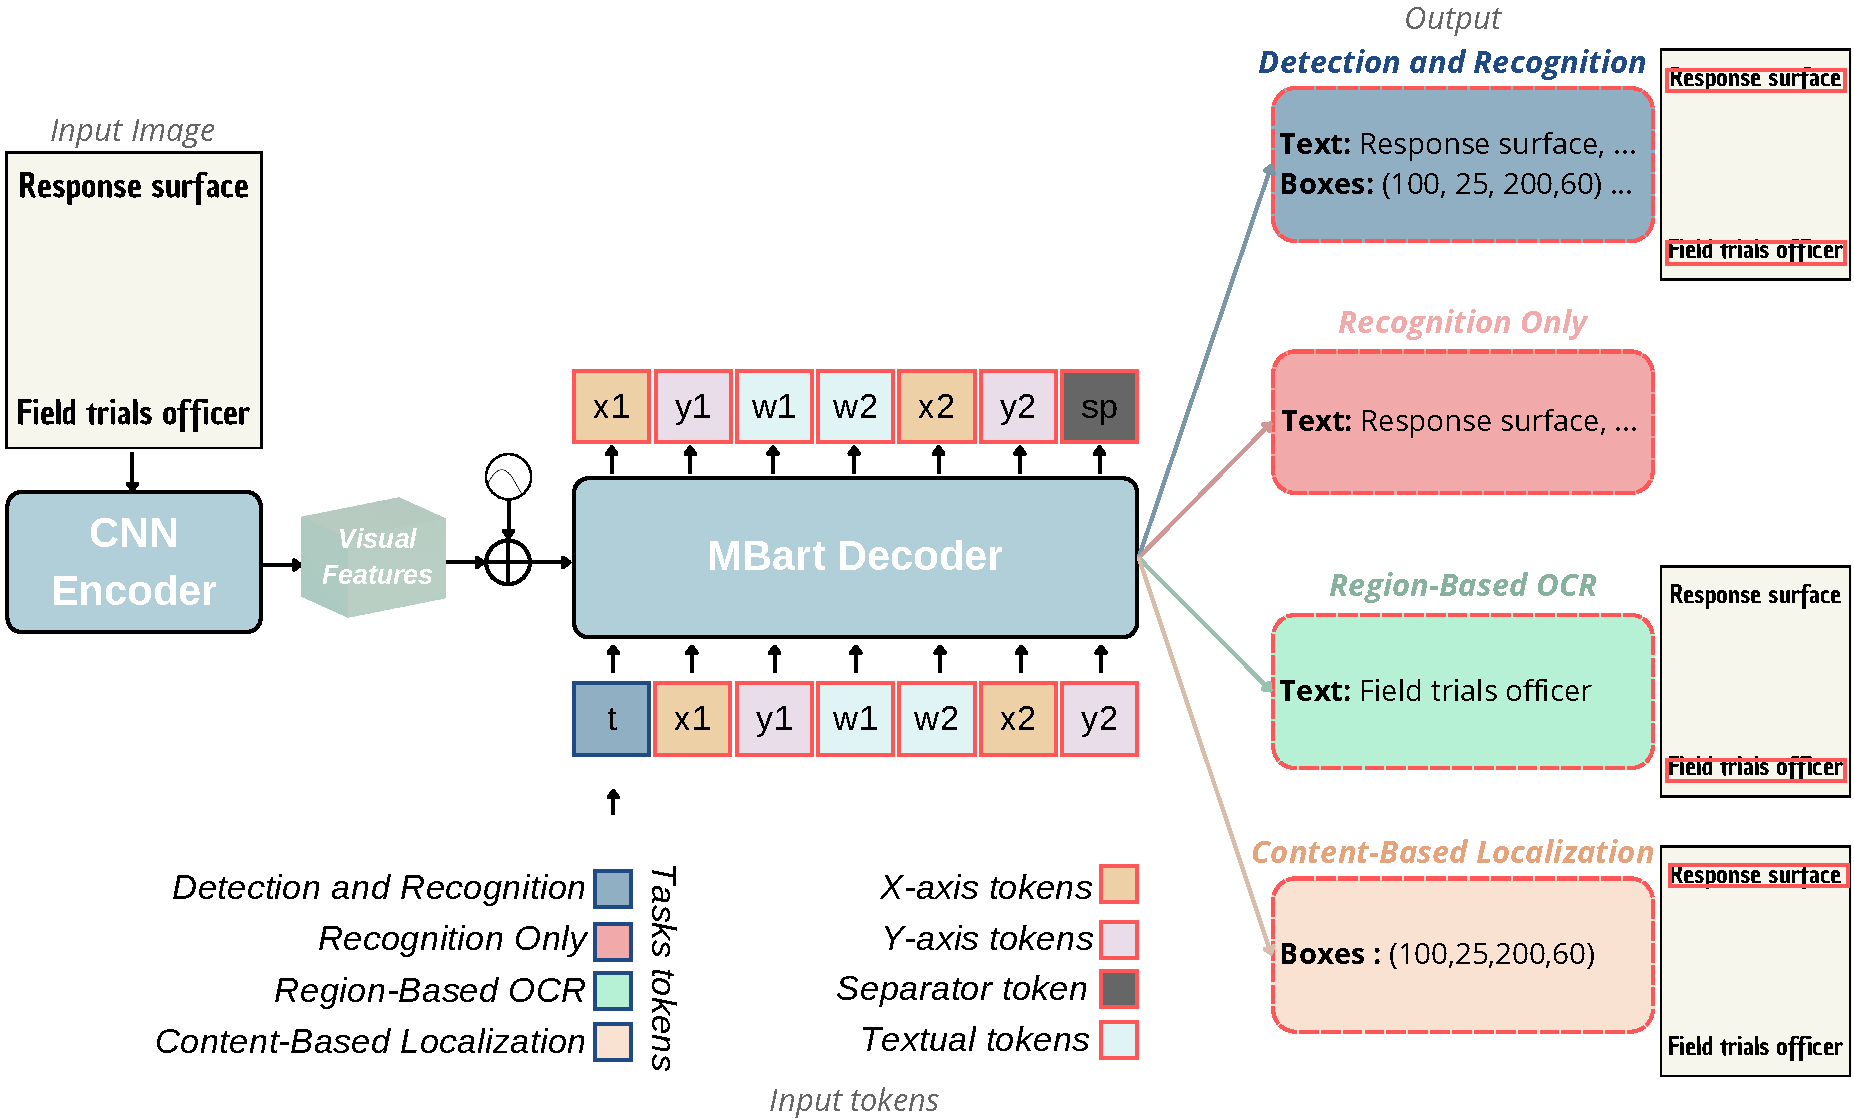
\includegraphics[width=0.4\textwidth]{pipeline.pdf} % Add the file name for your figure here
	\caption{Fine-Tuning Process Overview}
	\label{fig:piplelineofvistaOCR}
\end{figure}

\paragraph{Evaluation Strategy.} 
To comprehensively evaluate the improved OCR model, we propose assessing it on two key aspects: \textbf{text detection} and \textbf{text recognition}. For text detection, standard metrics such as Precision, Recall, and F1-score based on the Intersection over Union (IoU) between predicted and ground-truth bounding boxes will be used. For text recognition, we will rely on metrics like Character Error Rate (CER) and Word Accuracy (WA), which are widely adopted in OCR benchmarking. This dual evaluation approach ensures that the model not only locates text accurately but also reads it correctly in various Vietnamese poster contexts.

\subsection{Generating Images}

\subsubsection{Approach 1: Fine-tuning Generative Image Models}

One approach to generating high-quality, prompt-aligned images in Vietnamese is to fine-tune a pre-trained text-to-image model, such as a diffusion-based architecture (e.g., Stable Diffusion). In this approach, modifications are proposed at the level of the text encoder to better support the Vietnamese language.

\paragraph{Text Encoder Adaptation.} Since most diffusion models are pre-trained using English-language datasets and CLIP-based encoders, they struggle to fully understand Vietnamese prompts. To address this, we propose replacing or integrating the original text encoder with a Vietnamese language model such as PhoBERT \cite{nguyen2020phobertpretrainedlanguagemodels} or mT5 \cite{xue2021mt5massivelymultilingualpretrained}. These models are trained on large Vietnamese corpora and can significantly improve the understanding of Vietnamese input.

\paragraph{Training Considerations.} While this approach is relatively straightforward conceptually, it requires substantial computational resources and a large, diverse Vietnamese dataset to fine-tune the entire pipeline effectively. In particular, the latent space learned during pre-training may not generalize well to Vietnamese prompts, making high-quality dataset creation a critical component. The dataset should cover a wide variety of Vietnamese concepts, objects, and cultural contexts to ensure generalization.

\paragraph{Text Rendering with ControlNet \cite{controlnet2023}.} To enable text rendering (e.g., for poster generation), we propose incorporating ControlNet modules into the generation pipeline. There are two possible workflows:
\begin{itemize}
	\item \textbf{Sequential Generation:} First, generate an image using the diffusion model; then, apply image inpainting or control-based text insertion to overlay Vietnamese text onto the image.
	\item \textbf{Joint Generation:} Alternatively, ControlNet can be guided during the image generation process to synthesize images with embedded text directly aligned with the prompt. This requires designing control conditions such as text masks or bounding boxes during training or inference.
\end{itemize}

This method allows for greater control and flexibility when generating images that must include specific textual content. However, it also adds complexity to the pipeline and further increases the need for annotated data that includes visual text cues.

Overall, this approach offers a high-potential direction for creating culturally and linguistically aligned Vietnamese text-to-image systems, though it requires significant investment in data collection and training infrastructure.

\subsubsection{Apporach 2: Add conditions to SD via Controlnet.}

This pipeline generates culturally grounded Vietnamese poster-style images using Stable Diffusion (SD) with ControlNet and reference images. Instead of retraining SD, the approach adds modular control using ControlNet and enhances generation fidelity with real Vietnamese references. See Fig. \ref{fig:approach2} and Alg. \ref{alg:1}.

	\begin{algorithm}
		\caption{Vietnamese Poster Generation Pipeline}
		\label{alg:1}
		\textbf{Input:} $x$: user prompt \\
		\textbf{Output:} Stylized image $\hat{y}$ \\
		\textbf{Data:} VectorDB of Vietnamese references
		
		\begin{algorithmic}[1]
			\State $p \gets$ SystemPrompt $+$ UserPrompt
			\State $s \gets \text{LLM}(p)$ \Comment{parsed scene}
			\State $R \gets \text{VectorDB.search}(s)$ \Comment{retrieve references}
			\For{$r \in \{ \text{pose, cloth, bg} \}$}
			\State $C_r \gets \text{ControlNet}_r(R_r)$
			\EndFor
			\If{add\_text}
			\State $T \gets \text{ControlNet}_{\text{text}}(\text{glyph})$
			\EndIf
			\State $z \gets \text{SD}(C_{\text{pose}} \oplus C_{\text{cloth}} \oplus C_{\text{bg}} \oplus T \oplus p)$
			\If{RL enabled}
			\State $r \gets \text{RewardModel}(z)$
			\State Update model using $r$
			\EndIf
			\State \Return $z$
		\end{algorithmic}
	\end{algorithm}
	
Explanation of Pseudo-Code:
\begin{itemize}
	\item User Prompt is processed with a System Prompt to guide LLMs.
	\item LLMs parse the prompt into structured phrases (e.g., "couple eating Pho").
	\item These phrases are used to search a VectorDB, retrieving relevant Vietnamese reference images.
	\item The images are fed into multiple ControlNets (e.g., for pose, background, clothing).
	\item SD combines all signals and generates an image.
	\item A glyph-image ControlNet can optionally add text.
	\item A Reward model evaluates the image (optional RL feedback).
\end{itemize}

\begin{figure*}[h!]
	\centering
	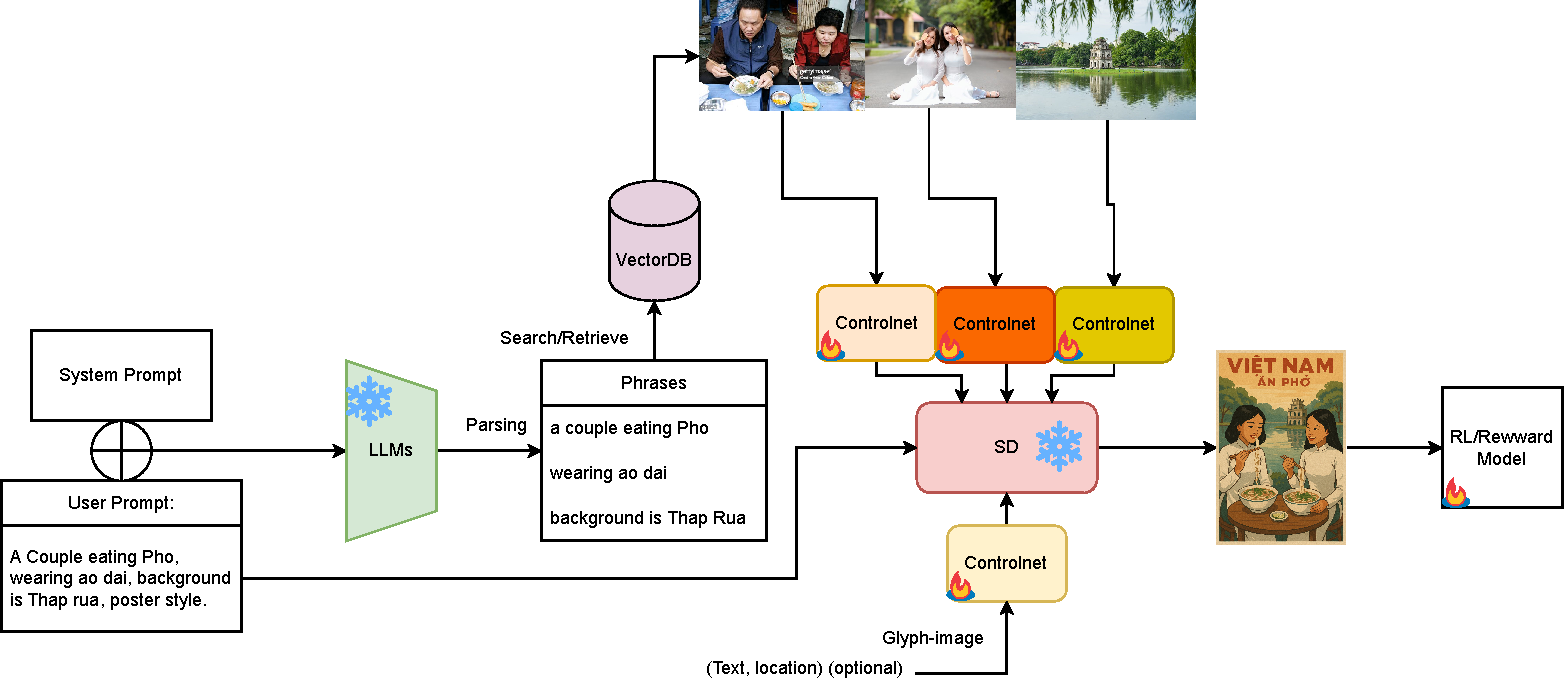
\includegraphics[width=1\textwidth]{diffusionproposal2.pdf} % Add the file name for your figure here
	\caption{Approach 2: Overview}
	\label{fig:approach2}
\end{figure*}

\paragraph{Prompt Parsing via Lightweight LLM}
To extract meaningful Vietnamese visual concepts from user prompts, we employ a lightweight large language model (LLM) with approximately 7 billion parameters. The model is guided by a fixed system prompt: 

\noindent\textbf{Prompt Template:}
{\small
	\begin{verbatim}
	You are a visual concept extractor for 
	Vietnamese cultural content in image captions. 
	Given a sentence, extract two types 
	of information:

	1. **Vietnamese Visual Keywords**: 
	iconic Vietnamese food, clothing, architecture, 
	festivals, or items.

	2. **Contextual Vietnamese Phrases**: 
	short phrases including actions or 
	descriptions involving Vietnamese 
	visual elements.

	Respond in JSON with two fields: 
	`keywords` and `phrases`.
	_____
	User: [User Prompt]
	\end{verbatim}
}

The LLM parses the user's natural language description into a structured JSON output containing two fields: \texttt{keywords} and \texttt{phrases}. For instance, given a prompt such as \textit{"A girl wearing ao dai, standing next to Cho Ben Thanh"}, the model may extract \texttt{"ao dai"} and \texttt{"Cho Ben Thanh"} as keywords, and \texttt{"a girl wearing ao dai"} as a contextual phrase. These parsed outputs are then used for querying a visual reference database in the next stage of the pipeline.

\paragraph{Image Retrieval via Phrase-based Embedding.} 
After extracting semantically rich Vietnamese visual phrases from textual prompts using a large language model (LLM), we embed these phrases into a shared image-text representation space using a retrained CLIP model tailored for Vietnamese cultural concepts. Unlike generic keyword-based search, our approach preserves contextual information (e.g., ``a couple eating Pho'' instead of simply ``Pho''), which enhances semantic alignment between text and images. These embedded phrases are used to retrieve the most relevant images from a large-scale image database via similarity search. The retrieved images—containing culturally significant visual elements—serve as visual conditions to guide a downstream generative model. Specifically, they are used as reference or conditioning inputs for a Stable Diffusion (SD) model, enabling it to generate images that are not only text-aligned but also visually grounded in authentic Vietnamese aesthetics and iconography.

\paragraph{Conditions for Diffusion.}
To enhance controllability and preserve visual faithfulness in image generation, we employ ControlNet modules to inject structured visual conditions into the diffusion process. The choice of ControlNet type depends on the nature of the extracted Vietnamese visual phrases. For instance, when the phrase includes human interactions such as ``a couple eating Pho,'' we utilize a pose-based ControlNet (e.g., OpenPose) to guide the human body layout and interaction. This ensures that the generated image captures realistic and culturally appropriate human gestures.

In cases where clothing elements such as ``ao dai'' are emphasized, we optionally combine pose ControlNet with a segmentation-based ControlNet (e.g., semantic segmentation or soft edge) to preserve the flowing structure and silhouette of traditional Vietnamese garments. This combination helps maintain the characteristic appearance of the ao dai in the generated imagery.

For background-specific elements like ``Thap Rua'' (Turtle Tower), we apply depth-based or canny-edge ControlNet modules. These models are effective in constraining architectural structures and spatial layouts, ensuring that the generated background remains faithful to the iconic landmark.

In addition to these visual conditions, we incorporate textual guidance—such as the original caption or refined visual phrases—using text-to-image capabilities or image inpainting when parts of the scene need to be conditionally completed or corrected.

Depending on the domain-specific requirements, these ControlNet models can either be used as-is (zero-shot) or fine-tuned on a curated dataset containing Vietnamese-specific visual patterns. For improved fidelity, we explore lightweight fine-tuning strategies (e.g., LoRA or DreamBooth) on each ControlNet branch to better adapt to cultural nuances and ensure consistency with the conditioning phrases.

\paragraph{Diffusion Model.}
Our final image synthesis step leverages a Stable Diffusion model conditioned on both visual control signals and user-defined prompts. The model receives multi-modal conditions from ControlNet—such as pose maps, edge maps, depth maps, or semantic segmentations—that encode structural and contextual information extracted from the original input. These control conditions act as spatial priors that constrain the generation process, allowing the model to produce images that are compositionally accurate and visually coherent.

Simultaneously, a natural language prompt provided by the user (e.g., ``a couple eating Pho in front of Thap Rua'') guides the model's semantic and stylistic output through cross-attention mechanisms within the diffusion architecture. This fusion of textual and structured visual conditions enables the model to generate high-fidelity images that are faithful to both the intended narrative and culturally specific visual details.

We build upon the Stable Diffusion 3 architecture, optionally extending it with ControlNet modules and fine-tuned LoRA weights to better align with Vietnamese aesthetics. This approach ensures that generated images not only follow the prompt accurately, but also integrate culturally meaningful elements like ``Pho'', ``ao dai'', and ``Thap Rua'' in a visually grounded and artistically coherent manner.

\paragraph{Reward Model.}
To further enhance the quality and cultural relevance of the generated images, we integrate a reward model based on Reinforcement Learning with Human Feedback (RLHF). The core idea is to fine-tune the diffusion process by introducing a classification model that evaluates whether the generated image contains distinctive Vietnamese cultural features. This classifier is trained with two classes: \textit{Vietnamese characteristic present} and \textit{Vietnamese characteristic absent}, based on a dataset of culturally rich images.

During the training phase, the reward model assesses the output of the Stable Diffusion model conditioned by ControlNet. If the generated image is classified as having strong Vietnamese characteristics (e.g., ``Pho'', ``Ao Dai'', or ``Thap Rua''), it receives a positive reward, encouraging the model to focus more on these cultural elements in future generations. Conversely, images that fail to capture these features are penalized. This feedback loop is utilized to refine the ControlNet conditioning process, leading to better optimization of the spatial and semantic conditions for culturally grounded image generation.

By using RLHF, we enable continuous improvements in the model's ability to align its outputs with both user prompts and culturally specific visual attributes, ensuring that the generated images maintain high fidelity to Vietnamese aesthetics while enhancing the overall quality and relevance of the generated content.

\paragraph{Model Evaluation.}
Evaluating the performance of a diffusion-based generative model is crucial to ensure that the generated images are both high-quality and culturally aligned with the desired attributes. To assess the effectiveness of our model, we employ a multi-faceted evaluation approach that includes both automated metrics (such as CLIP scores) and human feedback mechanisms.

Firstly, we leverage a CLIP-based evaluation method, where we utilize a CLIP model retrained on Vietnamese-specific data to compute similarity scores between the generated images and their corresponding textual prompts. This retrained CLIP model, which has been fine-tuned to recognize culturally relevant visual features (e.g., ``Pho'', ``Ao Dai'', and ``Thap Rua''), is capable of evaluating how well the model's output aligns with the semantic and visual cues embedded in the prompt. The CLIP score, a measure of cosine similarity between the image and text embeddings, serves as a quantitative metric for evaluating the degree of alignment between the generated content and the cultural context defined by the user’s prompt. Higher CLIP scores indicate better alignment with Vietnamese aesthetics and features, while lower scores highlight areas where the model may need further refinement in capturing cultural nuances.

In addition to CLIP-based evaluation, we also design a human feedback pipeline to assess the subjective quality and cultural fidelity of the generated images. This evaluation system allows human evaluators to rate the images on several key criteria, including but not limited to:
\begin{itemize}
	\item \textbf{Cultural Authenticity:} Does the image reflect Vietnamese cultural elements accurately (e.g., traditional attire like Ao Dai, famous landmarks like Thap Rua, or iconic foods like Pho)?
	\item \textbf{Visual Aesthetics:} Is the image visually pleasing, with proper lighting, composition, and realistic rendering?
	\item \textbf{Prompt Consistency:} How well does the image adhere to the given text prompt? Are the key elements of the prompt (e.g., "a couple eating Pho") clearly visible and well-represented in the image?
	\item \textbf{Clarity and Detail:} Are the image details sufficiently sharp, and does it avoid visual artifacts or blurring, especially in complex areas like faces or landmarks?
\end{itemize}

Evaluators rate each image on a scale from 1 to 5 for each criterion, with 1 indicating poor performance and 5 indicating excellent performance. These ratings are then aggregated to generate an overall quality score, which can be used to guide further refinements in the model's training process. This human-centered evaluation allows for a more nuanced understanding of how well the model performs in real-world scenarios, especially when it comes to cultural sensitivity and subjective visual preferences.

To optimize the model based on human feedback, we integrate the ratings from the human feedback pipeline into a reinforcement learning framework, specifically using Reinforcement Learning with Human Feedback (RLHF). The ratings from evaluators are treated as rewards or penalties for the model’s outputs, further refining the model’s ability to generate culturally accurate and aesthetically pleasing images. By incorporating both objective metrics (e.g., CLIP scores) and subjective human evaluation, we can ensure that the diffusion model produces outputs that are not only quantitatively accurate but also culturally relevant and visually appealing.

This dual evaluation approach—using both automated metrics and human feedback—provides a comprehensive framework for assessing the quality and relevance of the generated images. It ensures that the model is continuously improved and optimized for producing images that align with user expectations, both in terms of cultural fidelity and visual quality.

\section{Conclusion and Future Work}
\label{sec:conclusion}

In this article, we have conducted a comprehensive review and exploration of text-to-image generation with a strong focus on embedding rich Vietnamese cultural characteristics into the generative process. Beginning with a detailed analysis of existing general-purpose datasets and public Vietnamese datasets, we examined the limitations and potential of current image-captioning practices in constructing high-quality Vietnamese text-to-image (T2I) datasets. Furthermore, we reviewed the architecture and progression of modern diffusion-based text-to-image models, identifying both their strengths and cultural limitations when applied to underrepresented regions like Vietnam.

In the latter half of the paper, we proposed a structured and domain-specific pipeline aimed at enhancing the cultural fidelity of generated images. Central to this pipeline is a well-defined data taxonomy that classifies image content along several Vietnamese-specific dimensions: traditional customs, historical periods, regional diversity, festivals, and national identity. We expanded this taxonomy to cover specialized subsets, most notably a focused effort on visual representations of the Vietnam People's Army (VPA), which encapsulates decades of military evolution, diverse unit-specific imagery, and high-context cultural elements.

Our work also proposed a practical generation pipeline integrating scene parsing, reference retrieval, and control-guided generation based on multimodal alignment. This approach not only enables stylistically consistent and culturally aware generation but also provides a robust framework for training and evaluating future Vietnamese-centric diffusion models.

\vspace{0.5em}
\textbf{Future Work.} In the future, we plan to modularize this project by dividing the development into smaller, manageable components—such as focused dataset curation for each cultural domain (e.g., clothing, festivals, military), controlled model fine-tuning, and feedback-driven reward optimization—to evaluate feasibility at each step. By validating the cultural and generative quality incrementally, we aim to build a scalable foundation for a comprehensive Vietnamese T2I diffusion framework that can serve as both a creative tool and a digital archive of national identity.

\bibliographystyle{IEEEtran}
\bibliography{references}
\vspace{12pt}


\end{document}
